\documentclass[11pt]{article}
\usepackage[T1]{fontenc}
\usepackage[utf8]{inputenc}
\usepackage{amsmath,amssymb,amsthm,booktabs}
\usepackage[margin=1in]{geometry}
\usepackage{tikz}
\usetikzlibrary{arrows.meta,calc,positioning}
\usepackage{hyperref,xurl}
\hypersetup{colorlinks=true,linkcolor=blue!50!black,urlcolor=blue!50!black}
\newtheorem{theorem}{Theorem}[section]
\newtheorem{lemma}[theorem]{Lemma}
\newtheorem{proposition}[theorem]{Proposition}
\newtheorem{corollary}[theorem]{Corollary}
\theoremstyle{remark}
\newtheorem{remark}[theorem]{Remark}
\newcommand{\HH}{\mathbb H}
\newcommand{\Vol}{\operatorname{Vol}}
\newcommand{\ip}[2]{\langle #1,#2\rangle}
\newcommand{\OCT}{\mathcal O}
\newcommand{\DBL}{\mathcal D}
\newcommand{\CELL}{\mathcal C}
\title{Volumes and octahedral chains of ideal right-angled\linebreak hyperbolic four-polytopes}
\author{Coxeter Polytopes Research Project}
\date{18 October 2026}
\begin{document}
\maketitle
\begin{abstract}
The regular ideal right-angled 24-cell has volume $4\pi^2/3$ and is the
unique minimum-volume entirely ideal right-angled hyperbolic
four-polytope, by Kolpakov. We prove that the next distinct volume is
$8\pi^2/3$ and that its unique equality case is the reflection double
of the 24-cell across one octahedral facet. We also prove a structure
theorem without a volume assumption: if every facet is a regular
ideal octahedron or its triangular-face double, the polytope splits
along actual octahedral sections into a chain of regular 24-cells,
with opposite cuts in every intermediate cell. The equality theorem
uses a separate defect argument to establish this facet hypothesis.
The proof combines cusp geometry, a finite small-facet classification,
an elementary closed-surface argument, and Lorentz normal identities.
The restricted structure theorem does not assert a decomposition or
volume divisibility for arbitrary ideal right-angled four-polytopes.
\end{abstract}

\section{Statements and proof dependencies}
A polytope in this paper is convex, finite-sided, four-dimensional,
and of finite hyperbolic volume. It is \emph{entirely ideal} if every
vertex lies at infinity, and \emph{right-angled} if every dihedral
angle is $\pi/2$. Write $\CELL$ for the regular ideal right-angled
24-cell, $\OCT$ for its regular ideal octahedral facet, and $\DBL$
for the union of $\OCT$ with its reflection across a triangular
face. The polyhedron $\DBL$ has nine vertices, eight triangular
faces and three quadrilateral faces.

\begin{theorem}[The published minimum]\label{thm:minimum}
For every entirely ideal right-angled hyperbolic four-polytope $P$,
\[
 \Vol(P)\ge\frac{4\pi^2}{3},
\]
with equality exactly when $P$ is isometric to $\CELL$.
\end{theorem}
This is Kolpakov's theorem \cite[Theorem~3]{Kolpakov}. We recall the
volume and incidence formulas underlying it below. Our later
all-octahedral recognition argument also recovers its equality
statement once those formulas are given.

\begin{theorem}[The second volume and its equality case]\label{thm:gap}
If $P$ is entirely ideal and right-angled and $P\not\cong\CELL$, then
\[
 \Vol(P)\ge\frac{8\pi^2}{3}.
\]
Equality holds exactly for the union of $\CELL$ and its reflection
across an octahedral facet. Its f-vector is $(42,168,164,38)$.
\end{theorem}

The next theorem concerns a restricted class, with no assumed volume.
Its additional hypothesis is
\begin{equation}\label{eq:spectrum}
 \text{every facet of $P$ is isometric to $\OCT$ or $\DBL$.}
\end{equation}
The word ``isometric'' fixes the intrinsic geometry, not just the
numbers of faces. Equivalently one may assume the corresponding
combinatorial types and use three-dimensional right-angled rigidity.

\begin{theorem}[Octahedral cuts and chains]\label{thm:chain}
Suppose that $P$ satisfies \eqref{eq:spectrum}. Finitely many pairwise
disjoint regular ideal octahedral sections cut $P$ into regular ideal
right-angled 24-cells. If $P$ has $N$ facets of type $\DBL$, then
$N=8k$ for an integer $k\ge0$, and there are $k+1$ cells. Their
adjacency graph is a path. Two cuts incident to one cell use opposite
facets. Within this class the isometry type of an existing polytope
is determined by its number of cells, and
\[
 \Vol(P)=(k+1)\frac{4\pi^2}{3}.
\]
\end{theorem}
We classify existing polytopes under \eqref{eq:spectrum}; the theorem
does not assert existence for every prescribed path length.

The logical order matters. First we prove the gap by facet defects
and an injection of opposite cusp facets. Next, at volume $8\pi^2/3$,
we prove independently that exactly eight facets are $\DBL$ and all
others are $\OCT$. Only then do we apply the general chain theorem:
$N=8$ gives two cells and identifies the double. In particular, the
facet hypothesis is not inferred from the desired decomposition.

\subsection{Published inputs}
Kolpakov's Lemmas~1--2 give the incidence and volume formulas used
below. Proposition~5 states that an ideal right-angled
three-polyhedron with a $k$-gonal face has at least $2k$ vertices,
with equality exactly for the $k$-antiprism. Section~4.3, Case~D and
Figure~6 give the unique admissible nine-vertex case. The equality
reduction also uses the ten-vertex octahedrite in Figure~7: among the
ten-vertex types with only triangles and quadrilaterals it is the
unique admissible one, and the edge-adjacency graph of its four
quadrilaterals consists of two disjoint edges. The pentagonal
antiprism is treated separately. We use the standard right-angled
rigidity in dimension three to identify these combinatorial models
geometrically, as in Kolpakov's use of Andreev's theorem.

These are three-dimensional small-facet inputs. No classification
of arbitrary four-polytopes is used. Opposite-cusp injection,
equality-spectrum reduction, closed surfaces, actual cutting
sections and the chain theorem are proved here.

\section{Discrete volume and facet defect}
Write $v,e,r,f$ for the numbers of vertices, edges, ridges and facets of
$P$. An ideal vertex link is a Euclidean rectangular three-box. Counting
its vertices and edges and using Euler's identity gives
\[
 e=4v,\qquad r=3v+f,\qquad
 \sum_{R\in\Omega_2(P)} k(R)=12v,
\]
where $k(R)$ is the number of vertices of a ridge $R$. Define
\[
 W(P)=\sum_R(k(R)-3).
\]
It follows that
\begin{equation}\label{eq:discrete}
 W(P)=3(v-f)\in3\mathbb Z_{\ge0},\qquad
 \Vol(P)=\frac{\pi^2}{3}(v-f+4)
 =\frac{4\pi^2}{3}+\frac{\pi^2}{9}W(P).
\end{equation}
The latter identity is Kolpakov's volume formula; equivalently,
Gauss--Bonnet applied to the reflection orbifold uses
$\chi=1-f/2+r/4-e/8=(v-f+4)/4$.

Every facet $F$ is an ideal right-angled three-polyhedron. Its ideal
vertices have valency four, so, writing $v_F$ for their number, it has
$2v_F$ edges and $v_F+2$ polygonal faces. Its defect is
\begin{equation}\label{eq:facet}
 d(F):=v_F-6=\sum_{R\subset F}(k(R)-3),\qquad
 \sum_F d(F)=2W(P).
\end{equation}
Defect zero characterizes the regular ideal octahedron. A positive
defect facet has a nontriangular face of size $k\ge4$; the antiprism
bound $v_F\ge2k$ implies $d(F)\ge2$. In particular defect one does not
occur.

\section{Opposite cusp facets}
For a facet $F$, let $q(F)$ be its number of nontriangular faces and
$s(F)$ the number of its cusps whose intrinsic horospherical rectangle
is nonsquare. The latter condition does not depend on horosphere scale.

\begin{lemma}[Opposite-cusp injection]\label{lem:injection}
Suppose the smallest positive facet defect of $P$ is $m$, and $F$ has
positive defect. There are $q(F)+s(F)$ pairwise distinct positive-defect
facets other than $F$: its neighbors across nontriangular ridges, and
the facets opposite $F$ at its nonsquare cusps. Therefore
\begin{equation}\label{eq:budget}
 2W(P)\ge d(F)+m\bigl(q(F)+s(F)\bigr).
\end{equation}
In particular, when $d(F)=m$,
$2W(P)\ge m(1+q(F)+s(F))$.
\end{lemma}
\begin{proof}
A neighbor across a nontriangle contains that same nontriangle and is
not octahedral. Distinct ridges of $F$ have distinct neighboring facets,
since the intersection of two facets is a face.

At a cusp $x$ of $F$, the face of the rectangular three-box opposite
the $F$-face belongs to a facet $F_x$. The two rectangles are congruent.
If the rectangle of $F$ is nonsquare, so is that of $F_x$, which cannot
be the regular ideal octahedron.

The supporting hyperplanes of $F$ and $F_x$ are asymptotic and meet
at exactly the ideal point $x$. Hence the same $F_x$ cannot occur at
a second cusp of $F$, nor can it meet $F$ across any ridge. Thus all
facets in the two lists are distinct and differ from $F$. Each has
defect at least $m$. Summing their defects in \eqref{eq:facet} proves
the assertion.
\end{proof}

If $P\not\cong\CELL$, a positive-defect facet exists: otherwise $W=0$
in \eqref{eq:facet}, and the volume formula and Kolpakov's unique
minimum identify $P$ with $\CELL$.

\section{The two cusp-shape calculations}
\begin{lemma}\label{lem:antiprism}
The cusp rectangles of the ideal right-angled $k$-antiprism have
aspect ratio $2\cos(\pi/k)$. Thus for $k\ge4$ all $2k$ cusps
are nonsquare.
\end{lemma}
\begin{proof}
Set $\theta=\pi/k$, $c=\cos\theta$, and take positive square roots in
\[
 h^2=\frac{1-c}{1+c},\quad r^2=\frac{2c}{1+c},\quad
 b^2=\frac{2}{c(1+c)},\quad \mu^2=\frac{2(1-c)}{c}.
\]
Use Lorentz form $(-1,1,1,1)$. The two vertex rings have heights
$\pm h$, radius $r$, and angular offset $\theta$. At
$u=(1,r\cos\theta,r\sin\theta,h)$, the four incident normals are
\[
 N=(h,0,0,1),\quad M_0=(1,b,0,h),\quad
 M_2=(1,b\cos2\theta,b\sin2\theta,h),\quad
 L=(1,b\cos\theta,b\sin\theta,-h).
\]
Their squares are $r^2,\mu^2,\mu^2,\mu^2$. Adjacent products vanish;
the opposite pairs are parallel. The identities $bc=r$ and
$\mu=2h/r$ give
\[
 \frac{M_0+M_2}{\mu}=\frac2\mu u,\qquad
 \frac Nr+\frac L\mu=\left(\frac hr+\frac1\mu\right)u.
\]
For two opposite unit normals with sum $\kappa u$, their separation
on a fixed horosphere is proportional to $\kappa$. To see this,
send $u$ to infinity in the upper-half-space model; the mirrors become
parallel vertical planes with unit horizontal normals. The two
separations therefore have ratio
\[
 \frac{2/\mu}{h/r+1/\mu}
 =\frac{2r^2}{1+h^2}=2c.
\]
The antiprism symmetries are vertex-transitive. Finally $2c>1$ for
$k\ge4$ (and equals one for $k=3$).
\end{proof}

\begin{lemma}\label{lem:nine}
An ideal right-angled three-polyhedron with nine vertices has
$d=3$, $q=3$ and $s=3$.
\end{lemma}
\begin{proof}
The antiprism bound excludes pentagons and larger faces. The complete
published nine-vertex octahedrite list consists of one admissible type:
two ideal regular octahedra glued across a triangular face
\cite[Section~4.3, Case~D2 and Figure~6]{Kolpakov}. Rigidity makes
this identification geometric. The three gluing cusps have rectangles
formed by joining two squares, hence aspect two. The other six cusps
remain square. Its three nontriangular faces are quadrilaterals.
\end{proof}

\section{Universal exclusion of intermediate volumes}
\begin{lemma}\label{lem:two}
A positive-defect facet has at least two nontriangular faces. If it
has exactly two, it is an antiprism.
\end{lemma}
\begin{proof}
If its only nontriangle has size $k$, then $d=k-3$, whereas the
antiprism bound gives $d\ge2(k-3)$, a contradiction. If the two sizes
are $k\ge l\ge4$, then
\[
 d=(k-3)+(l-3)\ge2(k-3).
\]
Thus $k=l$ and equality holds in the antiprism bound; its equality
statement identifies the facet with $A_k$.
\end{proof}

\begin{proof}[Proof of the lower bound in Theorem~\ref{thm:gap}]
Choose a facet $F$ of smallest positive defect $m\ge2$.
Lemma~\ref{lem:injection} gives $2W\ge m(1+q+s)$.
The following cases are exhaustive.
\begin{enumerate}
\item If $F=A_k$, then $m=2k-6$, $q=2$, and
$s=2k=m+6$ by Lemma~\ref{lem:antiprism}. Hence
$2W\ge m(m+9)\ge22$.
\item A non-antiprism with $m=2$ is impossible: $v_F=8$ gives
$k\le4$ for every face, so its defect is two quadrilaterals and
Lemma~\ref{lem:two} applies.
\item If $m=3$, Lemma~\ref{lem:nine} gives $2W\ge3(1+3+3)=21$.
\item If $m=4$, every face has size at most five. A pentagon gives
equality in the antiprism bound and has already been treated. Otherwise
there are four quadrilaterals, so $2W\ge4(1+4)=20$.
\item If $m\ge5$ and $F$ is not an antiprism,
Lemma~\ref{lem:two} gives $q\ge3$, whence $2W\ge4m\ge20$.
\end{enumerate}
Thus $W\ge10$. Since $W$ is divisible by three, $W\ge12$.
Equation~\eqref{eq:discrete} proves the lower bound. In particular the
three prospective intermediate defects $3,6,9$, with respective
volumes $5\pi^2/3$, $2\pi^2$ and $7\pi^2/3$, cannot occur.
\end{proof}

\section{The intrinsic doubled octahedron}\label{sec:doubled}


The three vertices of the gluing face of $\DBL$ have a simple
intrinsic description: their horospherical rectangles are nonsquare.
At each of these vertices the rectangle is obtained by adjoining
two unit squares along one side, and therefore has aspect ratio two.
The remaining six rectangles are square. The three quadrilateral
faces of $\DBL$ meet pairwise at its three nonsquare cusps and have
no common edges. At a nonsquare cusp, the two quadrilateral sides
are the two long sides of its $2$ by $1$ rectangle.

The convex hull of the three nonsquare cusps is an ideal triangle
$T_F$ whose relative interior lies in the relative interior of a
doubled facet $F$. This is its
original gluing triangle. Each side of $T_F$ is the interior diagonal
of a quadrilateral face of $F$. At a nonsquare cusp, $T_F$ meets
the horospherical rectangle along the transverse segment halfway
along its long direction. Figure~\ref{fig:rectangle} records these
facts in the Euclidean link, where their metric meaning is literal.

\begin{figure}[htbp]
\centering
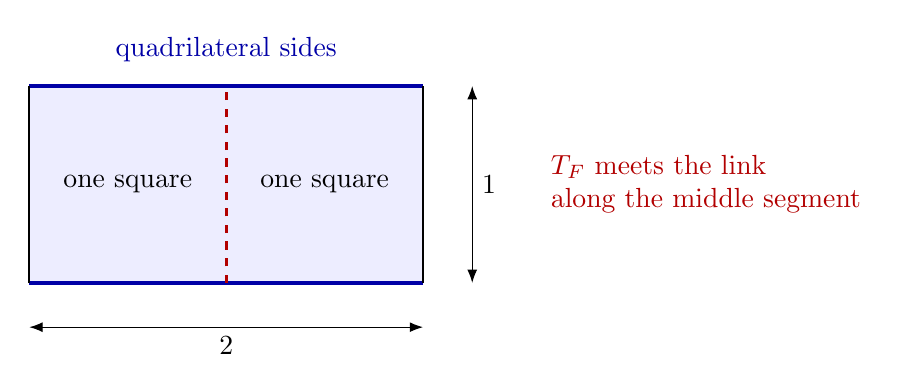
\begin{tikzpicture}[scale=1.25,>=Latex]
 \fill[blue!7] (0,0) rectangle (4,2);
 \draw[very thick,blue!65!black] (0,0)--(4,0) (0,2)--(4,2);
 \draw[thick] (0,0)--(0,2) (4,0)--(4,2);
 \draw[dashed,very thick,red!70!black] (2,0)--(2,2);
 \draw[<->] (0,-.45)--node[below] {$2$}(4,-.45);
 \draw[<->] (4.5,0)--node[right] {$1$}(4.5,2);
 \node at (1,1) {one square};
 \node at (3,1) {one square};
 \node[above,blue!65!black] at (2,2.15) {quadrilateral sides};
 \node[align=left,anchor=west,red!70!black] at (5.2,1)
 {$T_F$ meets the link\\along the middle segment};
\end{tikzpicture}
\caption{The cusp rectangle of a doubled octahedron at a gluing
vertex. The blue sides belong to its quadrilateral faces. The red
segment is the link of the internal triangle. This is an exact
Euclidean link diagram, not a perspective drawing of $\HH^4$.}
\label{fig:rectangle}
\end{figure}

At a square cusp of $\DBL$, exactly one incident polygonal face
is a quadrilateral. At a cusp of $\OCT$, none is. These facts will be used both in the equality reduction and in the
general octahedral cutting argument.

\section{The facet spectrum at the second volume}\label{sec:equalityspectrum}
In this section alone assume $\Vol(P)=8\pi^2/3$. Then $W=12$ and
$\sum_Fd(F)=24$. A facet is \emph{positive} when its defect is
positive; all others are regular ideal octahedra. Let $N$ be the
number of positive facets and $m$ their minimum defect. For any
positive facet, opposite-cusp injection gives the nonminimal form
\begin{equation}\label{eq:equalitybudget}
 24\ge d(F)+m\bigl(q(F)+s(F)\bigr).
\end{equation}
We shall prove the following statement before making any use of
Theorem~\ref{thm:chain}.
\begin{proposition}\label{prop:equalityspectrum}
There are exactly eight positive facets, each isometric to $\DBL$.
All other facets are isometric to $\OCT$.
\end{proposition}
For continuity with the small-facet list, we also write D9 for
$\DBL$. Its three quadrilateral faces have no common edges and
meet pairwise at its three nonsquare cusps. Every triangle contains
at most one of those cusps; the quadrilaterals contain two each,
as opposite vertices. At a square cusp exactly one incident face
is quadrilateral. These are the intrinsic facts of
Section~\ref{sec:doubled}.

\subsection{Acute intersections}


We use the following projection to pass from pairwise facet adjacency to actual common faces. Give every supporting wall a unit outward spacelike normal. Distinct wall products are nonpositive for an acute Coxeter chamber. If \(n_1,\dots,n_k\) are mutually orthogonal and \(p\) is a strict future timelike interior point, put

\[
 u=p-\sum_{i=1}^k\langle p,n_i\rangle n_i.
\]

Then \(u^2=p^2-\sum_i\langle p,n_i\rangle^2<0\), \(\langle u,n_i\rangle=0\), and every other wall product is strictly negative: each subtracted product \(\langle p,n_i\rangle\langle n_i,n_j\rangle\) is nonnegative. The projected timelike vector has the future sign, for example because \(\langle p,u\rangle=u^2<0\). Thus the k walls meet in an actual codimension-k face. Three mutually adjacent right-angled facets meet along an actual edge; four would give a finite vertex, forbidden here.

Consequently, if F has nontriangular neighbors G and H and G is adjacent to H anywhere in P, the corresponding two faces of F share an edge. This excludes an adjacency elsewhere that is invisible in the intrinsic facet picture.

\subsection{The minimum positive defect is three}\label{first-reduction-the-minimum-positive-defect-is-three}

\textbf{No antiprism \(A_k\) with \(k\ge5\).} Its defect is \(d=2k-6\ge4\), \(q=2\) and \(s=2k=d+6\). Even the universal \(m\ge2\) in \eqref{eq:equalitybudget} gives

\[
 24\ge d+2(d+8)=3d+16\ge28,
\]

a contradiction.

\textbf{No defect two facet.} Such a facet is the square antiprism A4. It has eight nonsquare cusps and two quadrilateral faces; each cusp belongs to exactly one of these quadrilaterals. If one face of a rectangular three-box is nonsquare, at least one of the other two opposite-face pairs is nonsquare. Otherwise both ratios to the third side would be one and all sides would be equal. Hence at each cusp of A4 at least two of its four ridge-neighbor facets are nonoctahedral. At most one is the unique quadrilateral neighbor through that cusp. At least one triangular neighbor is therefore positive. Covering the eight cusps by triangular faces requires at least three distinct such triangular neighbors. These are distinct from F, its two quadrilateral neighbors, and its eight nonsquare-cusp opposites, by the opposite-cusp injection. Thus at least 14 positive facets exist, giving total defect at least 28. This is impossible. We have \(m\ge3\).

\textbf{The branch \(m\ge5\) is impossible.} There are at most four positive facets. Every positive facet is a non-antiprism, so has at least three nontriangular faces. Their neighbors must be distinct positive facets. Thus there are exactly four, all pairwise adjacent. The acute-intersection fact would give a finite vertex.

\textbf{The branch \(m=4\) is impossible.} There are at most six positive facets. Choose a defect four facet \(F\). A pentagon would force A5, already excluded. Thus F is the Figure 7 ten-vertex octahedrite, with four quadrilaterals paired by edge adjacency. Let \(G_1,\dots,G_4\) be their four positive neighbors. The induced adjacency graph on these four neighbors is contained in that matching, by the acute-intersection fact. Each \(G_i\) has at most F, its one matching partner and one further positive facet as possible nontriangular neighbors. Every \(G_i\) needs at least three such neighbors, so a further facet must exist and \(q(G_i)=3\). None of the \(G_i\) can have defect four, since that case has four nontriangular faces; hence each has defect at least 5. Including F and the necessary further facet already gives \(4+4\cdot5+4=28\), a contradiction.

It follows that \textbf{\(m=3\)}, so some facet is D9.

\subsection{Exactly eight positive facets}\label{exactly-eight-positive-facets-all-d9}

A D9 facet and its three quadrilateral neighbors and three nonsquare-cusp opposites give seven positive facets. Since \(m=3\) and the total defect is 24,

\[
 7\le N\le8.
\]

If \(N=8\) all defects are three, as desired. Suppose \(N=7\). For every D9 facet, the seven just counted exhaust all positive facets. In particular:

\begin{quote}
Under \(N=7\), no triangular ridge of a D9 facet has a positive neighbor.
\end{quote}

The seven defects are at least three and sum to24. The possible excess partitions above seven copies of three are: one defect six; a defect five and a defect four; or three defects four. There are at most three facets whose defects exceed three.

There can be no defect four facet \(F\). Its four quadrilaterals occur in edge-adjacent pairs. Suppose one quadrilateral neighbor G were D9, and let H be the neighbor across its paired quadrilateral. The edge shared by the two quadrilaterals of F is an actual edge shared by F,G,H. In G, the faces cut out by F and H share this edge. The former is a quadrilateral. The latter cannot be a quadrilateral because D9's quadrilaterals share no edges, and cannot be a triangle because H is positive and \(N=7\) forbids a positive triangular neighbor. Thus every one of F's four quadrilateral neighbors would have defect greater than three. There are at most two such facets other than F, a contradiction.

We are left with one defect six facet \(F\) and six D9 facets. Every nontriangle of F is shared with a D9, and is therefore a quadrilateral. There are exactly six quadrilaterals. No two share an edge, by the same argument with their common D9 neighbor: two adjacent quadrilaterals of F would force either adjacent quadrilaterals or a positive triangular neighbor in D9.

The facet \(F\) has twelve vertices. Its six quadrilaterals give24 quadrilateral-vertex incidences. At a four-valent vertex no two consecutive faces can both be quadrilaterals; therefore there are at most two quadrilaterals there. Equality in the incidence count forces exactly two, alternating with two triangles, at every vertex. Form a graph J whose vertices are the six quadrilateral faces and whose edges are the twelve vertices of F, joining the two incident quadrilaterals. It is a simple 4-regular graph on six vertices: two distinct quadrilateral faces cannot share two vertices without sharing an edge, since their intersection is a face of the convex three-polyhedron. Its complement is a perfect matching, so it is the octahedral graph.

The embedding and medial recovery are explicit here. Draw each new edge from a center of one quadrilateral to their shared original vertex and then to the center of the other quadrilateral. Alternation at every original vertex makes this a spherical embedding, with the eight original triangular regions as its eight triangular faces. Those face cycles are distinct: a connected embedded graph with more than three vertices cannot have both sides of one $3$-cycle as faces, since then no other vertex or edge could lie on either side. The octahedral graph has exactly eight 3-cycles, so all its 3-cycles are precisely these faces. This determines the face incidences, not merely the abstract graph. Recover F with one vertex for each edge of J, its six quadrilaterals around the six vertices of J, and its eight triangles around those eight 3-cycles. This is exactly the cuboctahedral face lattice. No general embedding-rigidity theorem or unbounded facet census is being assumed.

The ideal right-angled cuboctahedron has all twelve cusp rectangles nonsquare, of aspect \(\sqrt2\). An exact model in Lorentz coordinates has vertices

\[
 (1,x),\quad x\text{ a permutation of }(\pm1,\pm1,0)/\sqrt2;
\]

its six square-wall normals are \((1,\pm\sqrt2 e_i)\), of norm one, and its eight triangle-wall normals are \((1,(\pm1,\pm1,\pm1)/\sqrt2)\), of norm \(1/2\). At \((1,1/\sqrt2,1/\sqrt2,0)\), the two opposite square normals sum to \((2,\sqrt2,\sqrt2,0)\), and the two opposite \emph{unnormalized} triangle normals have the same sum. Unit normalization multiplies the latter by \(\sqrt2\). The horospherical width ratio is therefore \(\sqrt2\), and symmetry gives it at every vertex. The model is the cube \(|X_i|\le1\) truncated by \(\sum|X_i|\le2\) in scaled Klein coordinates, so its combinatorics are explicit. Right-angled rigidity identifies F with this model.

The opposite-cusp injection for F would now give \(1+6+12=19\) positive facets, contradicting \(N=7\). We conclude:

\[
 \boxed{N=8,\quad d(F)=3\text{ for every positive facet}.}
\]

All other facets are regular ideal octahedra. All nontriangular ridges are quadrilaterals; there are twelve of them.

\section{Cusp boxes under the octahedral facet hypothesis}\label{sec:chainproof}
We now drop the volume assumption of Section~\ref{sec:equalityspectrum}
and assume only \eqref{eq:spectrum}. In particular $W$ need not be12
and the number of doubled facets need not be eight. We prove
Theorem~\ref{thm:chain} directly from this intrinsic facet geometry.

\begin{lemma}\label{lem:box}
Every noncubic cusp box of $P$ has side proportions $2:1:1$.
Its four nonsquare faces belong to doubled facets and form a belt;
its two square end faces belong to ordinary octahedral facets.
Every adjacency within the belt is a quadrilateral ridge of $P$.
\end{lemma}
\begin{proof}
Each face rectangle of a cusp box is intrinsic to a facet of $P$.
Its aspect ratio is therefore one or two. If the three side lengths
were distinct, the ratio of the largest to the smallest would exceed
two, since the two consecutive unequal ratios must both be two.
Thus a noncubic box has proportions $2:1:1$ or $2:2:1$.

Consider a $2:2:1$ box. The four nonsquare faces must be doubled
facets. In each, the two long sides are quadrilateral sides. Each
square end face consequently has four incident quadrilateral sides.
An octahedral cusp has none, and a square cusp of a doubled facet
has exactly one. Neither permitted facet type can supply an end
face. The $2:2:1$ box is impossible.

In a $2:1:1$ box, the four long rectangles are the belt. Their
mutual sides are the long sides and hence are quadrilateral ridges.
The square ends meet the belt only along its short, triangular
sides. All four incidences at an end are triangular, so the end
cannot be a square cusp of a doubled facet. It is octahedral.
\end{proof}

\section{The internal triangles form closed surfaces}

Join two doubled facets when they share a quadrilateral ridge.
The distinguished triangles in these facets have the same internal
diagonal in that ridge, so we glue them along this diagonal. The
gluing is geometrically defined; there is no choice of an abstract
edge identification.

\begin{lemma}\label{lem:surface}
After adjoining their ideal vertices, the glued triangles form a
finite closed two-manifold. Its connected components are exactly
the components of the quadrilateral adjacency graph of doubled facets.
Every edge lies in two triangles and every vertex lies in four.
\end{lemma}
\begin{proof}
The interior of a distinguished triangle lies in the relative
interior of its facet. Interiors of different facets are disjoint.
An edge of the triangle is in the relative interior of an actual
quadrilateral ridge, which lies in precisely two facets. Thus each
edge has two incident triangles and has a disk neighborhood at
each of its finite points.

It remains to check the ideal vertices. By Lemma~\ref{lem:box},
the triangles incident to one such point come from the four doubled
facets in a single $2:1:1$ belt. Their four middle segments join
end to end around the box, giving the simple square shown in
Figure~\ref{fig:belt}. They do not cross and do not leave an open
end. This square is the link of the point in the glued surface.
Coning the link gives a disk after the ideal point is adjoined.
There are no other triangle vertices.

All four doubled facets at such a vertex are already connected
through their quadrilateral belt. Therefore identifying ideal
vertices does not join two different components of the quadrilateral
adjacency graph. The components of the graph and of the surface
coincide.
\end{proof}

\begin{figure}[htbp]
\centering
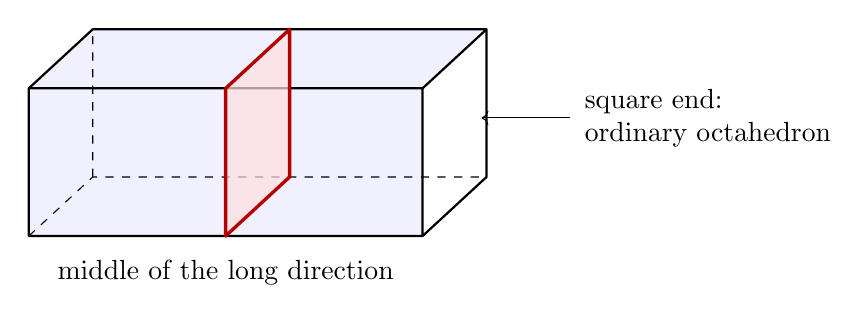
\begin{tikzpicture}[scale=1.25,line join=round]
 \coordinate (A) at (0,0); \coordinate (B) at (4,0);
 \coordinate (C) at (4,1.5); \coordinate (D) at (0,1.5);
 \coordinate (E) at (.65,.6); \coordinate (F) at (4.65,.6);
 \coordinate (G) at (4.65,2.1); \coordinate (H) at (.65,2.1);
 \fill[blue!6] (A)--(B)--(C)--(G)--(H)--(D)--cycle;
 \draw[thick] (A)--(B)--(C)--(D)--cycle (B)--(F)--(G)--(C)
 (D)--(H)--(G);
 \draw[dashed] (A)--(E)--(F) (E)--(H);
 \fill[red!12,opacity=.7] (2,0)--(2.65,.6)--(2.65,2.1)--(2,1.5)--cycle;
 \draw[very thick,red!70!black] (2,0)--(2.65,.6)--(2.65,2.1)--(2,1.5)--cycle;
 \node[below] at (2,-.15) {middle of the long direction};
 \draw[->] (5.5,1.2)--(4.6,1.2);
 \node[anchor=west,align=left] at (5.55,1.2)
 {square end:\\ordinary octahedron};
\end{tikzpicture}
\caption{Four internal triangles meet an ambient $2:1:1$ cusp box
in its transverse middle square. Its boundary is the four-segment
link used to prove that the compactified triangle complex is a
two-manifold. The filled square indicates the transverse section;
only its boundary lies on the box surface.}
\label{fig:belt}
\end{figure}

\begin{lemma}\label{lem:euler}
A connected component containing $n$ triangles contains exactly
eight triangles, twelve edges and six vertices.
\end{lemma}
\begin{proof}
Write $e$ and $v$ for its edge and vertex counts. The incidence
counts of Lemma~\ref{lem:surface} give
\[
 e=\frac{3n}{2},\qquad v=\frac{3n}{4},\qquad
 \chi=v-e+n=\frac n4.
\]
We shall use only the elementary inequality $\chi\le2$ for a
connected closed cellulated surface; we do not assume the surface
is a sphere. Here is a direct proof in the present setting.
Choose a spanning tree $A$ of its one-skeleton. Delete from the
dual graph the edges dual to $A$. The remaining dual graph is
connected. Otherwise, the boundary between one nonempty proper
set of triangular faces and its complement would be a nonempty
subgraph of $A$. At each vertex its degree is even: a walk around
the circular link enters and leaves the chosen set equally often.
This gives a nonempty Eulerian subgraph of a tree, which is
impossible. We may therefore choose a dual spanning tree disjoint
from $A$. The two trees use $v-1$ and $n-1$ distinct edges, so
$e\ge v+n-2$ and $\chi\le2$. It follows that $n\le8$, and the
integer $\chi=n/4$ also shows that $n$ is divisible by four.

We next obtain a lower bound within the same component. Choose
one doubled facet $F$. Its three quadrilateral faces have three
distinct doubled neighbors. Its three nonsquare cusps also have
three opposite doubled facets. The latter are distinct from one
another and from every ridge neighbor: their walls are asymptotic
to the wall of $F$ at exactly one specified ideal point, whereas
a ridge neighbor intersects its wall along a plane. These opposite
facets belong to the same component, because opposite belt members
are connected by the four-cycle of quadrilateral adjacencies.
Together with $F$ we have found seven distinct facets in the
component. Thus $7\le n\le8$ and $4\mid n$, forcing $n=8$.
The values of $e$ and $v$ follow.
\end{proof}

\section{From six cusps to eight wall normals}

Fix one component. Make a graph $J$ whose six vertices are its
cusps and whose edges are the twelve internal diagonals. Every
vertex has degree four.

\begin{lemma}\label{lem:graph}
The graph $J$ is the octahedral graph. Its eight triangles are the
eight distinguished facet triangles. The doubled facets can
therefore be indexed by $s\in\{\pm1\}^3$ so that quadrilateral
adjacency changes exactly one sign.
\end{lemma}
\begin{proof}
First, $J$ has no parallel edges. If two different quadrilateral
ridges joined the same two cusps, their incident facets would
include at least three of the four belt members at either cusp.
Among three belt members there are two opposite ones. Their walls
are asymptotic at that cusp and cannot contain the second cusp.
This is a contradiction. Two distinct ridges cannot have the same
pair of incident facets, since the intersection of two convex
facets is one face. Thus $J$ is simple.

A simple four-regular graph on six vertices has complement a
perfect matching, so it is the octahedral graph. Each distinguished
triangle gives a three-cycle in $J$. Two facets cannot give the
same three-cycle: its geometric triangle would then have an
interior point in the relative interiors of two different facets.
The octahedral graph has exactly eight three-cycles, obtained by
choosing one vertex from each of its three opposite pairs. All
eight occur. Label these opposite pairs by $1,2,3$, with a sign
on each member. A triangle, and hence a doubled facet, is indexed
by its three choices of sign. Two triangles share an edge exactly
when one sign changes.
\end{proof}

\begin{figure}[htbp]
\centering
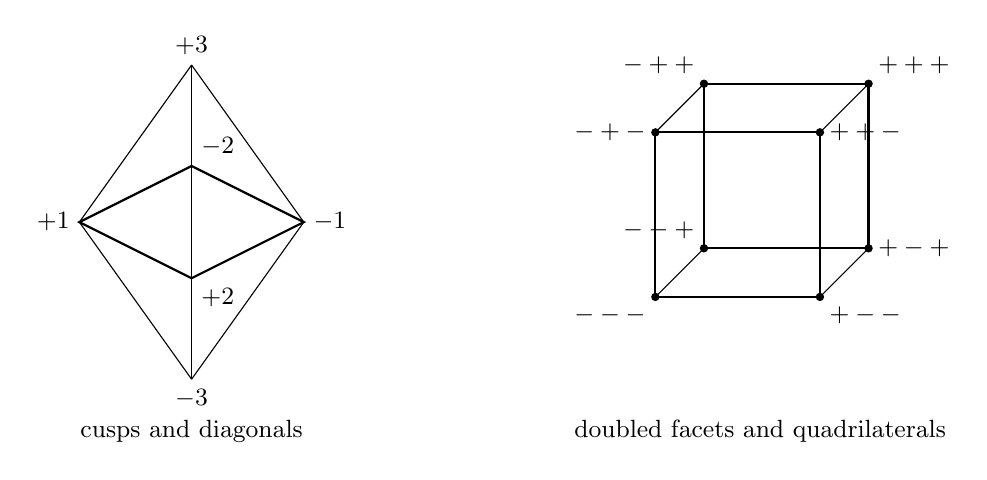
\begin{tikzpicture}[scale=.95,every node/.style={font=\small}]
 \coordinate (xp) at (-1.5,0); \coordinate (yp) at (0,-.75);
 \coordinate (xm) at (1.5,0); \coordinate (ym) at (0,.75);
 \coordinate (zp) at (0,2.1); \coordinate (zm) at (0,-2.1);
 \draw[thick] (xp)--(yp)--(xm)--(ym)--cycle;
 \foreach \p in {xp,yp,xm,ym}{\draw (zp)--(\p) (zm)--(\p);}
 \node[left] at (xp) {$+1$}; \node[right] at (xm) {$-1$};
 \node[below right] at (yp) {$+2$}; \node[above right] at (ym) {$-2$};
 \node[above] at (zp) {$+3$}; \node[below] at (zm) {$-3$};
 \node at (0,-2.8) {cusps and diagonals};
 \begin{scope}[xshift=6.2cm,yshift=-1cm]
 \coordinate (a) at (0,0); \coordinate (b) at (2.2,0);
 \coordinate (c) at (2.2,2.2); \coordinate (d) at (0,2.2);
 \coordinate (e) at (.65,.65); \coordinate (f) at (2.85,.65);
 \coordinate (g) at (2.85,2.85); \coordinate (h) at (.65,2.85);
 \draw[thick] (a)--(b)--(c)--(d)--cycle (e)--(f)--(g)--(h)--cycle;
 \draw (a)--(e) (b)--(f) (c)--(g) (d)--(h);
 \foreach \p/\lab/\pos in {a/{---}/below left,b/{+--}/below right,
 c/{++-}/right,d/{-+-}/left,e/{--+}/above left,f/{+-+}/right,
 g/{+++}/above right,h/{-++}/above left}
 {\fill (\p) circle (1.6pt);\node[\pos] at (\p) {$\lab$};}
 \node at (1.4,-1.8) {doubled facets and quadrilaterals};
 \end{scope}
\end{tikzpicture}
\caption{The two incidence graphs. The six-cusp graph is octahedral;
its eight triangles index the doubled facets. The dual cube records
quadrilateral adjacency. The signs specify which cusp from each
opposite pair belongs to a distinguished triangle. These are
incidence drawings, not metric projections of the polytope.}
\label{fig:graphs}
\end{figure}

\section{Equal widths put the triangles in one hyperplane}

We work in $\mathbb R^{4,1}$ with form
$\ip{x}{x}=-x_0^2+x_1^2+\cdots+x_4^2$. A wall has an outward
unit spacelike normal $n$, and its halfspace is $\ip{x}{n}\le0$.
Let $n_s$ be the normals of the eight doubled facets just indexed.

\begin{lemma}\label{lem:width}
On each square of the cube in Figure~\ref{fig:graphs}, the sums of
the two opposite pairs of normals agree.
\end{lemma}
\begin{proof}
The square is a cusp belt. Its opposite wall pairs bound the two
short directions of the $2:1:1$ box, so their Euclidean separations
on a common horosphere agree. The use of unit normals matters.
With cusp null vector $\xi=(1,0,0,0,1)$, the vertical wall $x_i=a$
in upper-half-space has unit normal $(a,e_i,a)$. The opposite wall
$x_i=b$, with the other outward orientation, has normal
$(-b,-e_i,-b)$. Their sum is $(a-b)\xi$. Thus its coefficient is
the separation, with the same normalization for both pairs. Equal
widths give equal sums.
\end{proof}

\begin{lemma}\label{lem:normal}
There are mutually orthogonal vectors $a,b_1,b_2,b_3$ such that
\[
 n_s=a+s_1b_1+s_2b_2+s_3b_3,\qquad
 a^2=-\tfrac12,\quad b_i^2=\tfrac12.
\]
\end{lemma}
\begin{proof}
The equations of Lemma~\ref{lem:width} say that every mixed second
finite difference on the cube vanishes. Expanding $s\mapsto n_s$
in sign characters leaves only its constant and three linear
terms, giving the displayed affine expression. Expanding the
eight equations $n_s^2=1$ and comparing sign characters gives
\[
 \ip{a}{b_i}=0,\quad \ip{b_i}{b_j}=0\ (i\ne j),\quad
 a^2+b_1^2+b_2^2+b_3^2=1.
\]
Adjacent facets meet orthogonally. If $s'$ differs from $s$ only
in coordinate $i$, then
$0=\ip{n_s}{n_{s'}}=1-2b_i^2$. Thus every $b_i^2=1/2$, and
the remaining identity gives $a^2=-1/2$.
\end{proof}

The span $U$ of these four vectors is Lorentzian and has dimension
four. Its orthogonal complement is a spacelike line. The
intersection of $U$ with $\HH^4$ is a genuine hyperbolic
hyperplane $H$, orthogonal to all eight doubled-facet walls.
In orthonormal coordinates on $U$, the wall normals are
$(1,s_1,s_2,s_3)/\sqrt2$, with the future sign determined by their
positive cusp-null sums. Their halfspaces cut out
\begin{equation}\label{eq:section}
 S=\{(t,x)\in\HH^3:|x_1|+|x_2|+|x_3|\le t\},
\end{equation}
the regular ideal octahedron. Its six null rays are $a\pm b_i$.
They are exactly the actual cusps of the component, because the
opposite belt-normal sums are $2(a\pm b_i)$.

Convexity now supplies the step that an abstract graph cannot:
since these six ideal points belong to the closure of $P$, their
hyperbolic convex hull $S$ is contained in $P$. Conversely the
eight actual facet inequalities imply $P\cap H\subset S$.
Therefore
\[
 P\cap H=S.
\]
Each face of $S$ is its facet's distinguished internal triangle.
Each edge of $S$ is the internal diagonal of an actual
quadrilateral ridge, as illustrated in Figure~\ref{fig:diagonal}.

\begin{figure}[htbp]
\centering
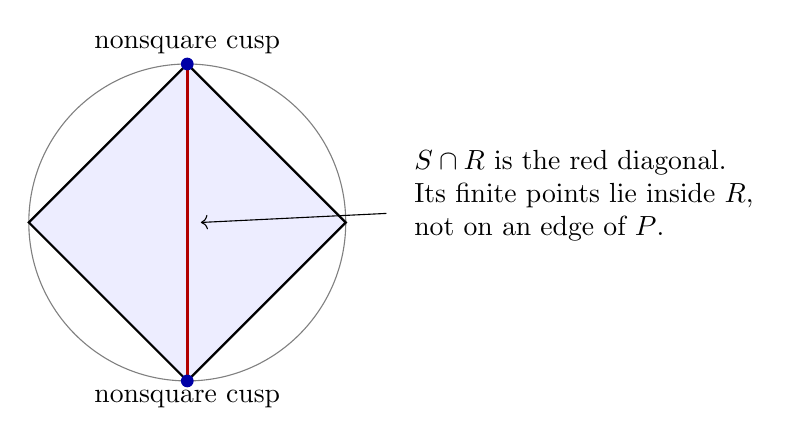
\begin{tikzpicture}[scale=1.15]
 \draw[gray] (0,0) circle (1.75);
 \coordinate (a) at (0,1.75); \coordinate (b) at (1.75,0);
 \coordinate (c) at (0,-1.75); \coordinate (d) at (-1.75,0);
 \fill[blue!7] (a)--(b)--(c)--(d)--cycle;
 \draw[thick] (a)--(b)--(c)--(d)--cycle;
 \draw[very thick,red!70!black] (a)--(c);
 \fill[blue!65!black] (a) circle (2pt) (c) circle (2pt);
 \node[above] at (a) {nonsquare cusp};
 \node[below] at (c) {nonsquare cusp};
 \node[anchor=west,align=left] at (2.4,.3)
 {$S\cap R$ is the red diagonal.\\Its finite points lie inside $R$,\\
 not on an edge of $P$.};
 \draw[->] (2.2,.1)--(.15,0);
\end{tikzpicture}
\caption{A quadrilateral ridge $R$ in the Klein disk. Its two
nonsquare cusps are opposite vertices. Their diagonal is an edge
of the cutting octahedron. This distinction is what prevents an
unrelated facet from touching the section at a finite edge point.}
\label{fig:diagonal}
\end{figure}

\section{Why the hyperplane is a legitimate cut}

\begin{lemma}\label{lem:cut}
No facet outside the chosen eight meets $S$ at a finite point.
Cutting along $H$ gives two finite-volume entirely ideal
right-angled four-polytopes. The eight doubled facets become
ordinary octahedra; every other facet is uncut.
\end{lemma}
\begin{proof}
Let $F$ be any outside facet. Its supporting functional is
nonpositive on $S$. If it vanishes at a relative interior point
of a face of $S$, it vanishes on that face. A finite point of $S$
lies in its interior, in a triangular face interior, or in an
edge interior. A triangular face interior belongs to the relative
interior of one of the chosen doubled facets, so it cannot belong
to $F$. An edge interior lies in the relative interior of a ridge
whose only two incident facets are the chosen doubled facets.
It cannot belong to $F$ either. A supporting functional vanishing
at an interior point would contain all of $S$, contradicting the
face-interior case. Thus $F$ has no finite intersection with $S$.

If $F$ crossed $H$, a finite segment in $F$ would meet
$P\cap H=S$ at a finite point. Consequently no outside facet
crosses. The chosen eight facets are cut along their genuine
gluing triangles into octahedra. The center of $S$ is strict on
all eight wall inequalities and, by what was just proved, on
every other wall inequality. It is an interior point of $P$;
both halves have nonempty interior.

In the Klein model, a vertex of a half lying on $H$ must be a
vertex of $S$. Otherwise it lies in a nontrivial segment of $S$
and is not extreme. Away from $H$, a vertex is an old vertex of
$P$. The only vertices of $S$ are its six old ideal cusps, so
no finite vertex is introduced. The new facet $S$ meets only the
eight cut walls, all orthogonal to $H$. Every new dihedral angle
is right; all other angles are inherited. Finite volume follows
by containment in $P$.
\end{proof}

The facet spectrum \eqref{eq:spectrum} is preserved by the cut.
There are exactly eight fewer doubled facets, counted over both
pieces. Repeating the construction therefore terminates.

There is also a useful geometric disjointness statement. Every
outside doubled facet lies on one side of the first cut. Two
quadrilateral-adjacent outside facets cannot lie on opposite
sides, since their shared ridge would give a finite intersection
with $S$. Thus a whole other component lies on one side. Its
section, being the convex hull of its six cusps, lies on that
side as well. A noncubic cusp belongs to only one belt component
and has octahedral ends; two sections cannot share an ideal
vertex. The outside-facet argument excludes finite boundary
contact. Hence the sections are pairwise disjoint, including
their ideal endpoints.

\section{Recognizing a piece with only octahedral facets}

We give a direct recognition argument rather than using a
four-dimensional classification as a final black box.

\begin{lemma}\label{lem:recognition}
An entirely ideal right-angled four-polytope whose facets are all
isometric to $\OCT$ is isometric to $\CELL$.
\end{lemma}
\begin{proof}
Place one facet $F$ on a facet of a model regular 24-cell. Its
eight triangular faces agree with those of the model facet.
For any one of these triangles, the adjacent supporting wall is
uniquely determined by the triangle and orthogonality to $F$'s
wall: its outward normal is the intrinsic outward unit normal
of that triangle within $F$'s wall.

In this adjacent wall, its octahedral facet is determined by the
shared ideal triangle and the side on which it lies. To justify
this last assertion, take any isometry between two regular ideal
octahedra with that triangular face. Every isometry of the face
extends to a symmetry of the octahedron, so the isometry can be
adjusted to fix the face vertices pointwise. An isometry of
$\HH^3$ fixing three distinct ideal points is the identity or
reflection in their plane; the specified side selects the
identity. The neighboring facet is therefore the whole model
octahedron, not only a piece on the same wall.

Repeat across its faces. The facet adjacency graph of the model
24-cell is connected. The propagation matches all 24 model
facets, with their full vertex sets, to actual facets of the
piece. Their halfspaces put the piece inside the model cell.
Conversely the closure of the piece contains every ideal model
vertex, and convexity contains their hull, the model cell.
The two polytopes agree.
\end{proof}

Each final piece is consequently a 24-cell. If the original
polytope has $N$ doubled facets, Lemma~\ref{lem:euler} gives
$N=8k$. Each of the $k$ cuts increases the number of pieces by
one, so there are $k+1$ cells. Their adjacency graph is a tree:
starting with one piece, each separating cut replaces one vertex
of the current adjacency tree by two vertices joined by one edge.

\section{Why the tree is a chain}

The restriction on facet types has one more consequence. In the
Lorentz model a regular 24-cell has outward unit normals
\[
 (1,r),\qquad
 r\in\{(\pm1,\pm1,0,0)\text{ and all coordinate permutations}\}.
\]
The spatial vectors are the roots of $D_4$. Distinct roots have
dot products $-2,-1,0,1$, with $-2$ only for opposite roots.

\begin{lemma}\label{lem:opposite}
If a cell in the decomposition meets two cutting sections,
these are opposite facets of that cell.
\end{lemma}
\begin{proof}
The sections have disjoint closures. If their roots are $r_1,r_2$,
then $r_1\cdot r_2$ is negative: dot product one gives an actual
common triangular ridge, and dot product zero gives a common
ideal vertex. Thus the dot product is $-1$ or $-2$.

Suppose it is $-1$. The vector $r_1+r_2$ is another $D_4$ root,
and its cell facet $Q$ is orthogonal to both cut walls, since
\[
 -1+(r_1+r_2)\cdot r_i=0\qquad(i=1,2).
\]
It cannot itself be a cutting facet, since it meets the two
sections along triangles. It is part of an original facet of $P$.
Across each of the two cuts there is a neighboring regular
24-cell. Its corresponding facet is the reflection of $Q$ and
lies in the same original supporting wall, because that wall is
orthogonal to the cut. This neighboring facet cannot be another
internal cut: it meets the first cut along a triangle, whereas
all cuts have disjoint closures. Thus the original facet contains
three regular ideal octahedra.

Their relative interiors are disjoint. If two had an open
overlap, a point of that overlap avoiding every other cell wall
would have an inward normal collar contained in both cells.
Their four-dimensional interiors would overlap, which is
impossible for pieces obtained by cuts. The original facet has
intrinsic volume at least three times $\Vol(\OCT)$; it can be
neither $\OCT$ nor $\DBL$. This contradicts
\eqref{eq:spectrum}. Hence the dot product is $-2$, and the two
facets are opposite.
\end{proof}

No cell can have three pairwise opposite facets. The adjacency
tree has maximum degree two and is a path. Once an end cell and
its first gluing facet are placed, every next cell is its
reflection across the gluing facet, and the next gluing facet in
an intermediate cell is uniquely the opposite one.

For completeness, there is no independent gluing twist. The
regular 24-cell is flag-transitive. Given an isometry of an
octahedral facet, send one facet flag to its image by a cell
symmetry. This symmetry stabilizes the facet and has the required
restriction, because an octahedral isometry fixing a flag is the
identity. Thus every facet symmetry extends to the cell.
Two cells on opposite sides of the same facet are therefore
uniquely placed up to the ambient reflection. This proves the
isometry assertion in Theorem~\ref{thm:chain}.

\begin{figure}[htbp]
\centering
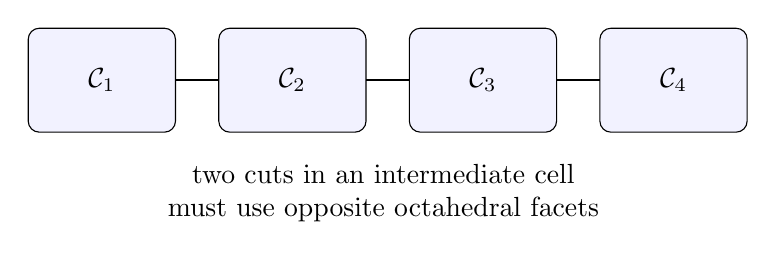
\begin{tikzpicture}[>=Latex,scale=1.1]
 \foreach \i in {0,1,2,3}{
  \draw[rounded corners,fill=blue!5] (2.2*\i,0) rectangle +(1.7,1.2);
  \node at (2.2*\i+.85,.6) {$\CELL_{\the\numexpr\i+1\relax}$};}
 \foreach \i in {0,1,2}{\draw[thick] (2.2*\i+1.7,.6)--(2.2*\i+2.2,.6);}
 \node[align=center] at (4.1,-.7)
 {two cuts in an intermediate cell\\must use opposite octahedral facets};
\end{tikzpicture}
\caption{The resulting adjacency graph is a path. The boxes denote
whole 24-cells and are not metric four-dimensional drawings. The
opposition condition comes from the common-neighbor argument in
Lemma~\ref{lem:opposite}, rather than from the drawing.}
\label{fig:chain}
\end{figure}

\section{Volume, face counts, and the limit of the result}

The regular ideal 24-cell has volume $4\pi^2/3$.
Volume additivity proves the formula in Theorem~\ref{thm:chain}. The common defect identities also give
$2W=3N=24k$, consistently with \eqref{eq:discrete}.

If there are $m=k+1$ cells, the complete face counts are
\[
 (v,e,r,f)=(18m+6,\ 72m+24,\ 68m+28,\ 14m+10).
\]
Indeed each gluing identifies six ideal vertices and removes two
facets while merging eight neighboring pairs. There are no extra
vertex identifications between nonadjacent cells: a common cusp
would lie on every separating cut along their path, whereas
different sections have no common ideal vertex. The edge and
ridge formulas then follow from the incidence identities above.
There are $8(m-1)$ doubled facets, $6m+18$ ordinary facets and
$12(m-1)$ quadrilateral ridges. All other ridges are triangles.
For $m=2$ this recovers $(42,168,164,38)$.

These formulas do not establish the same quantization for arbitrary
ideal right-angled four-polytopes. Without
\eqref{eq:spectrum}, a facet may have more complicated cusp
rectangles, the internal triangles used here may not exist, and
the local links need not be the four-segment belts of
Lemma~\ref{lem:surface}. A successful extension must replace those
geometric facts, not merely repeat the Euler count.

\section{Equality and attainment}\label{sec:attainment}
\begin{proof}[Equality in Theorem~\ref{thm:gap}]
If $\Vol(P)=8\pi^2/3$, Proposition~\ref{prop:equalityspectrum}
puts $P$ in the Oct/D class and gives $N=8$. Theorem~\ref{thm:chain}
therefore gives $k=1$: there are exactly two regular 24-cells joined
across one octahedral facet. The placement and no-twist argument in
the chain proof shows that they are mutual reflections in that
facet. Conversely their reflection double is an entirely ideal
right-angled polytope of twice the 24-cell volume, as the explicit
construction below verifies. This proves the equality assertion.
\end{proof}

\subsection{An exact model of the attaining double}

In Lorentz form $(-1,1,1,1,1)$, take the 24 unit normals $(1,a)$,
where $a$ runs through the $D_4$ roots having exactly two nonzero
entries, each $\pm1$. In the time-one Klein section their ideal
vertices are the eight $\pm e_i$ and the sixteen
$(\pm\tfrac12,\pm\tfrac12,\pm\tfrac12,\pm\tfrac12)$.
The inequalities are $|x_i|+|x_j|\le1$; they are bounded and their
origin is strict. Exact enumeration of all $\binom{24}{4}=10,626$
active four-wall subsets verifies that the displayed vertices are all
vertices of the intersection.

Reflect across $n=(1,1,1,0,0)$ by
$x\mapsto x-2\ip{x}{n}n$. Remove the gluing wall from both cells
and identify coincident walls. The resulting 38 halfspaces contain
the union. Indeed, for an old wall normal $m\ne n$ and $x\in\CELL$,
\[
 \ip{x}{s_n(m)}=\ip{x}{m}-2\ip{m}{n}\ip{x}{n}\le0,
\]
since both $\ip{m}{n}$ and $\ip{x}{n}$ are nonpositive. The
mirrored containment follows by reflection. Conversely, on each side of the gluing hyperplane, their
inequalities together with that side's gluing inequality include all
inequalities of the corresponding original cell. Thus the new
intersection equals the union. In particular no unexamined escape
directions or additional vertices are being discarded.

The interiors are disjoint, so the volume is twice $4\pi^2/3$.
The exact face reconstruction supplies the following independent
incidence check.
\begin{center}
\begin{tabular}{lrr}
\toprule Quantity&24-cell&Double\\\midrule
Vertices&24&42\\ Edges&96&168\\ Ridges&96&164\\ Facets&24&38\\
Triangular ridges&96&152\\ Quadrilateral ridges&0&12\\
Octahedral facets&24&30\\ Doubled-octahedron facets&0&8\\
Ridge defect $W$&0&12\\ Reflection-orbifold Euler characteristic&1&2\\
\bottomrule
\end{tabular}
\end{center}
Each of the eight doubled-octahedron facets has nine vertices, eighteen
edges, eight triangles and three quadrilaterals. There are six shared
cusps and 36 other cusps. Every cusp has six incident facets, eight
edges and twelve ridges. The facet--vertex check is
$30\cdot6+8\cdot9=6\cdot42$. This completes attainment and
the construction of the equality model.

\appendix
\section{Finite data and verification scope}
The universal gap proof uses the published volume formula, the
antiprism bound and the stated nine-vertex classification. The
equality-spectrum proof adds only the ten-vertex Figure~7 entry and
three-dimensional rigidity; it proves the cuboctahedral alternative
and excludes it by its cusp widths. The general chain proof does
not assume a four-dimensional minimum classification: it constructs
actual sections, proves their disjointness, and recognizes every
all-octahedral piece by propagation in the explicit 24-cell model.

The finite supporting data have narrower purposes. The reflected
double certificate checks exact rational walls, vertices, ridges,
facets and cusp links. The equality certificate checks the small
incidence transcriptions, the cuboctahedral model and cusp widths,
the simple four-regular six-vertex graph possibilities, and cube
normal identities. The $D_4$ root checker verifies the finite
24-cell root/vertex and reflected-octahedron facts used in the
opposition argument. None of these finite model checks replaces
opposite-cusp injection, the equality reductions, the surface proof,
or convexity and actual-face arguments.

The source maps and solver-free commands are recorded in
\path{docs/result_manuscript_correspondence.md} and
\path{manuscripts/catalogue.json}. The older separate sources are
preserved proof inputs. Conditional Lean interfaces distinguish the
published minimum, the internal defect partition, the independent
equality-spectrum reduction, the one-cut geometry and final gluing.
They do not supply an end-to-end formal proof of the hyperbolic
geometry by assuming the final volume or decomposition conclusion.

\begin{thebibliography}{9}
\bibitem{Kolpakov}
A.~Kolpakov, \emph{On the optimality of the ideal right-angled 24-cell},
Algebraic \& Geometric Topology \textbf{12} (2012),1941--1960.
\href{https://doi.org/10.2140/agt.2012.12.1941}{doi:10.2140/agt.2012.12.1941}.
\end{thebibliography}
\end{document}
